\subsection{IR radiation source}
\label{subsec:ir:radiation-source}

The IRPD measurements for characterising the infrared signature of ionic complexes in this study are performed with two types of infrared (IR) radiation sources, the free-electron lasers FELIX and an optical parametric oscillator/amplifier (OPO/A) system. In this section, we shall briefly describe the interface of the FELion ion-trap instrument with these IR radiation sources.

\begin{figure}[!htb]
    \centering

    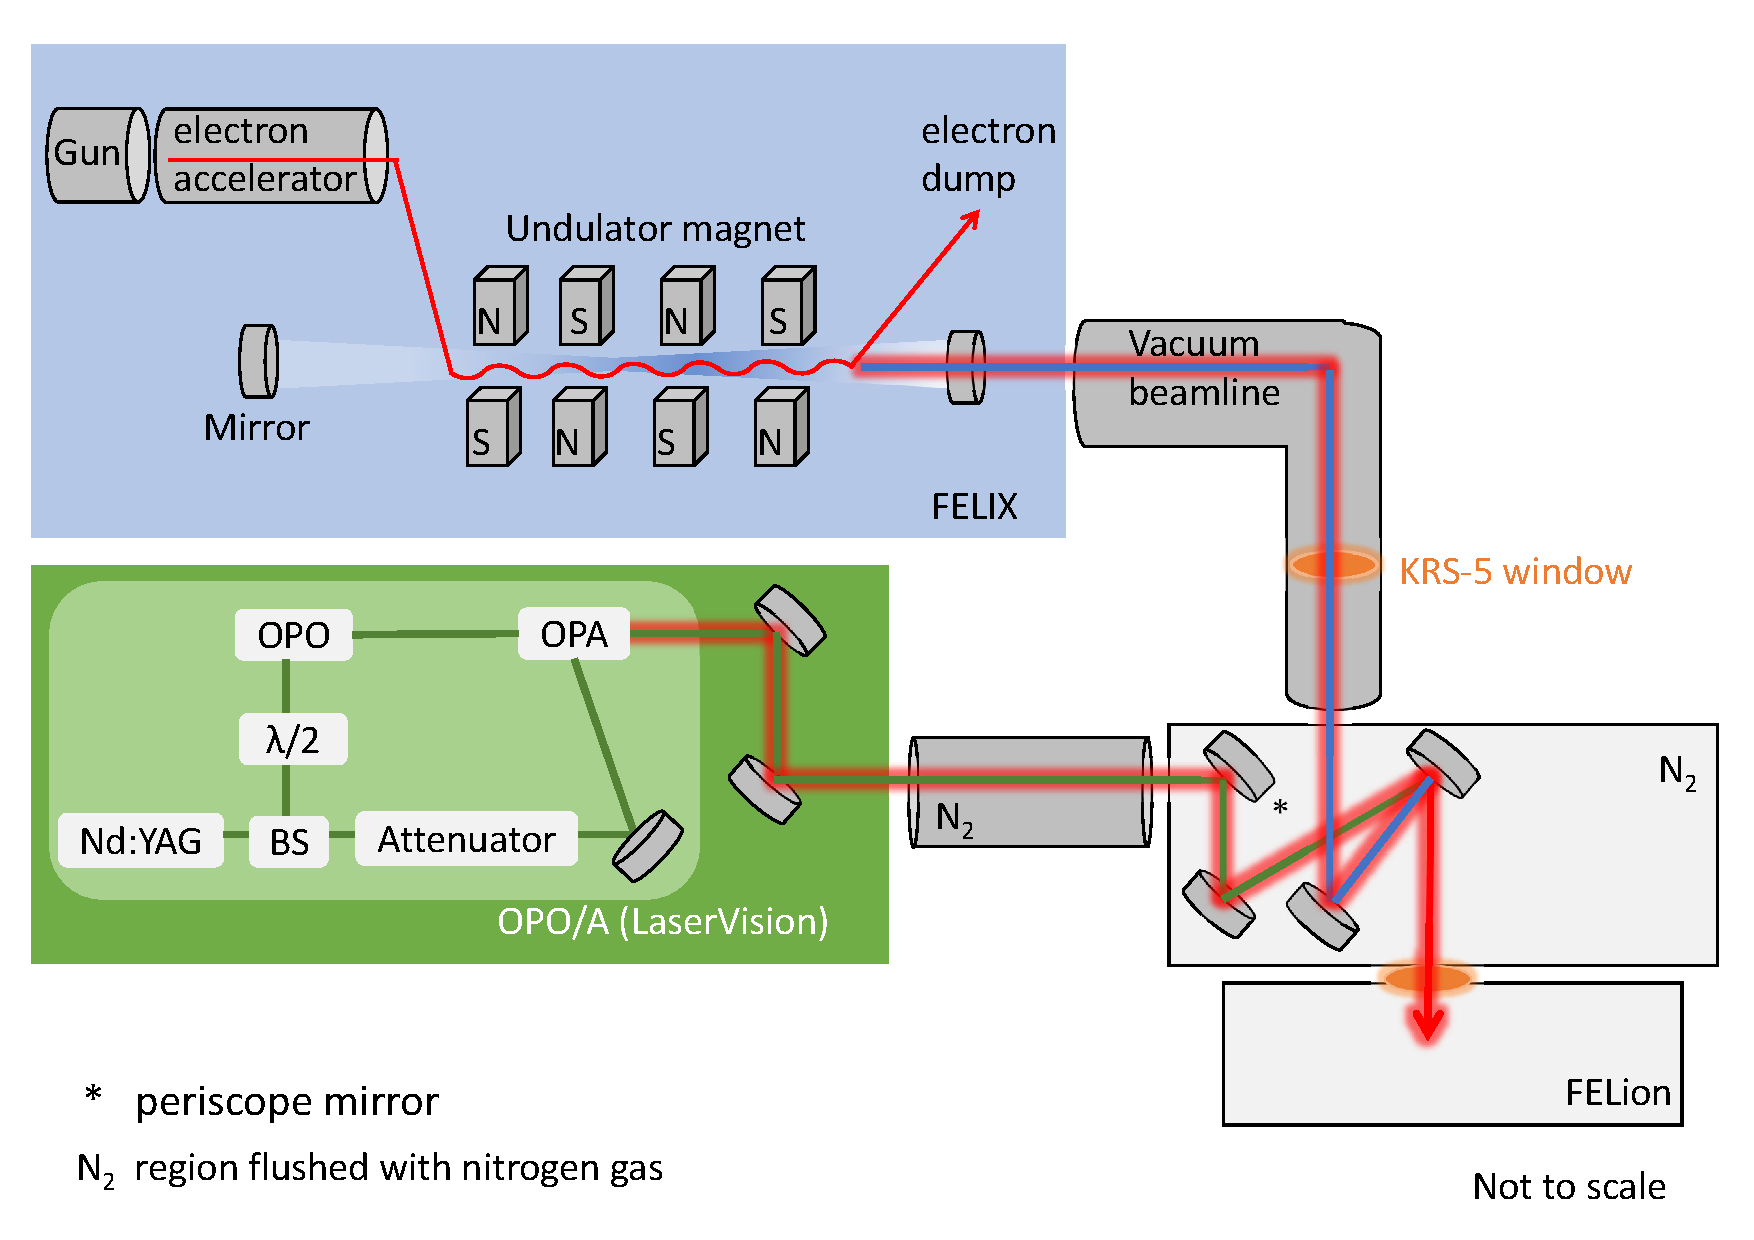
\includegraphics[width=1\textwidth]{figures/Instruments/FELIX-OPO-beamline.pdf}
    \caption{Schematic drawing of FELIX and OPO/A system interfaced with FELion user-station. The blue and green coloured lines represent the FELIX and OPO/A output laser beam paths, respectively. Only one system, FELIX or OPO/A, is operated at a given time.}
    \label{fig:FELIX}
\end{figure}

\subsubsection{FELIX} 
\label{subsec:ir:radiation-source:FELIX}

FELIX stands for \qt{Free Electron Lasers for Infrared eXperiment}; as the name suggests, it is a free-electron laser (FEL) facility, and the FELion instrument is located in its user-stations \cite{jusko_felion_2019}. This section briefly introduces the operating principles of an FEL, followed by a detailed description of the FELIX laser system coupled to the FELion instrument used in this study for infrared experiments.\\

\textbf{Operating principles:} In a conventional laser device, the laser light is generated through optical amplification based on the stimulated emission of electromagnetic radiation from e.g. an atomic or a molecular excitation. A free-electron laser system however employs relativistic electrons as a gain medium. As shown in Figure \ref{fig:FELIX}, an electron accelerator provides a beam of relativistic electrons followed by an undulator (periodic arrangement of magnets with alternating poles) in which the electrons perform a transverse oscillation and travel along the axis of the undulator. Two highly reflective mirrors form an optical laser resonator in which the radiation is amplified. By adjusting the electron beam's energy or the magnetic field strength of the undulator, the wavelength of the radiation emitted, $\lambda_r$ can be easily tuned and is given by \cite{oepts_free-electron-laser_1995}:

\[\lambda_r = \frac{\lambda_u}{2\gamma^2} \enclose{1 + \frac{K^2}{2}}\]

where $\lambda_u$ is the undulator wavelength (spatial period of the magnetic field), $\gamma$ is the relativistic Lorentz factor, and $K$ is the dimensionless parameter describing undulator magnetic strength.

The $\gamma$ and $K$ are defined as:
\begin{align*}
    \begin{split}
        \gamma &= \frac{1}{\sqrt{1-(v_z/c)^2}}\\
        K &= \frac{eB_u\lambda_u}{2\pi m_e c}
    \end{split}
\end{align*}
where $v_z$ is the velocity of the electron in the direction of the undulator, $c$ is the speed of light, $m_e$ is the mass of the electron, $e$ is the elementary charge, and $B_u$ is the applied magnetic field strength.\\

\textbf{FELIX laser system:} Currently, the FELIX laboratory consists of four laser systems, FEL-1, FEL-2, FELICE, and FLARE, each producing their range of wavelengths, and together, they provide a tuning range of 3-1500 $\mu$m. The FELion instrument is interfaced with the FEL-1 and FEL-2 pulsed IR laser system via an evacuated beamline with a wide tunable frequency range of 30-150 $\mu$m (330-66 \wn) and 3-45 $\mu$m (3330-220 \wn), respectively. FEL-2 delivers $> 2000$ \wn\ in $3^{rd}$ harmonic operation mode (FEL-2 was updated in 2022 after the experiments reported in this thesis have been concluded). The IR pulsed FELIX laser has a repetition rate of 10 Hz with a typical macropulse length of $\sim  10\ \mu$s and for the experiments reported here a 1 GHz micro-pulse structure (see Figure \ref{fig:FELIX-pulse}) has been used. 

\begin{figure}[!htb]
    \centering
    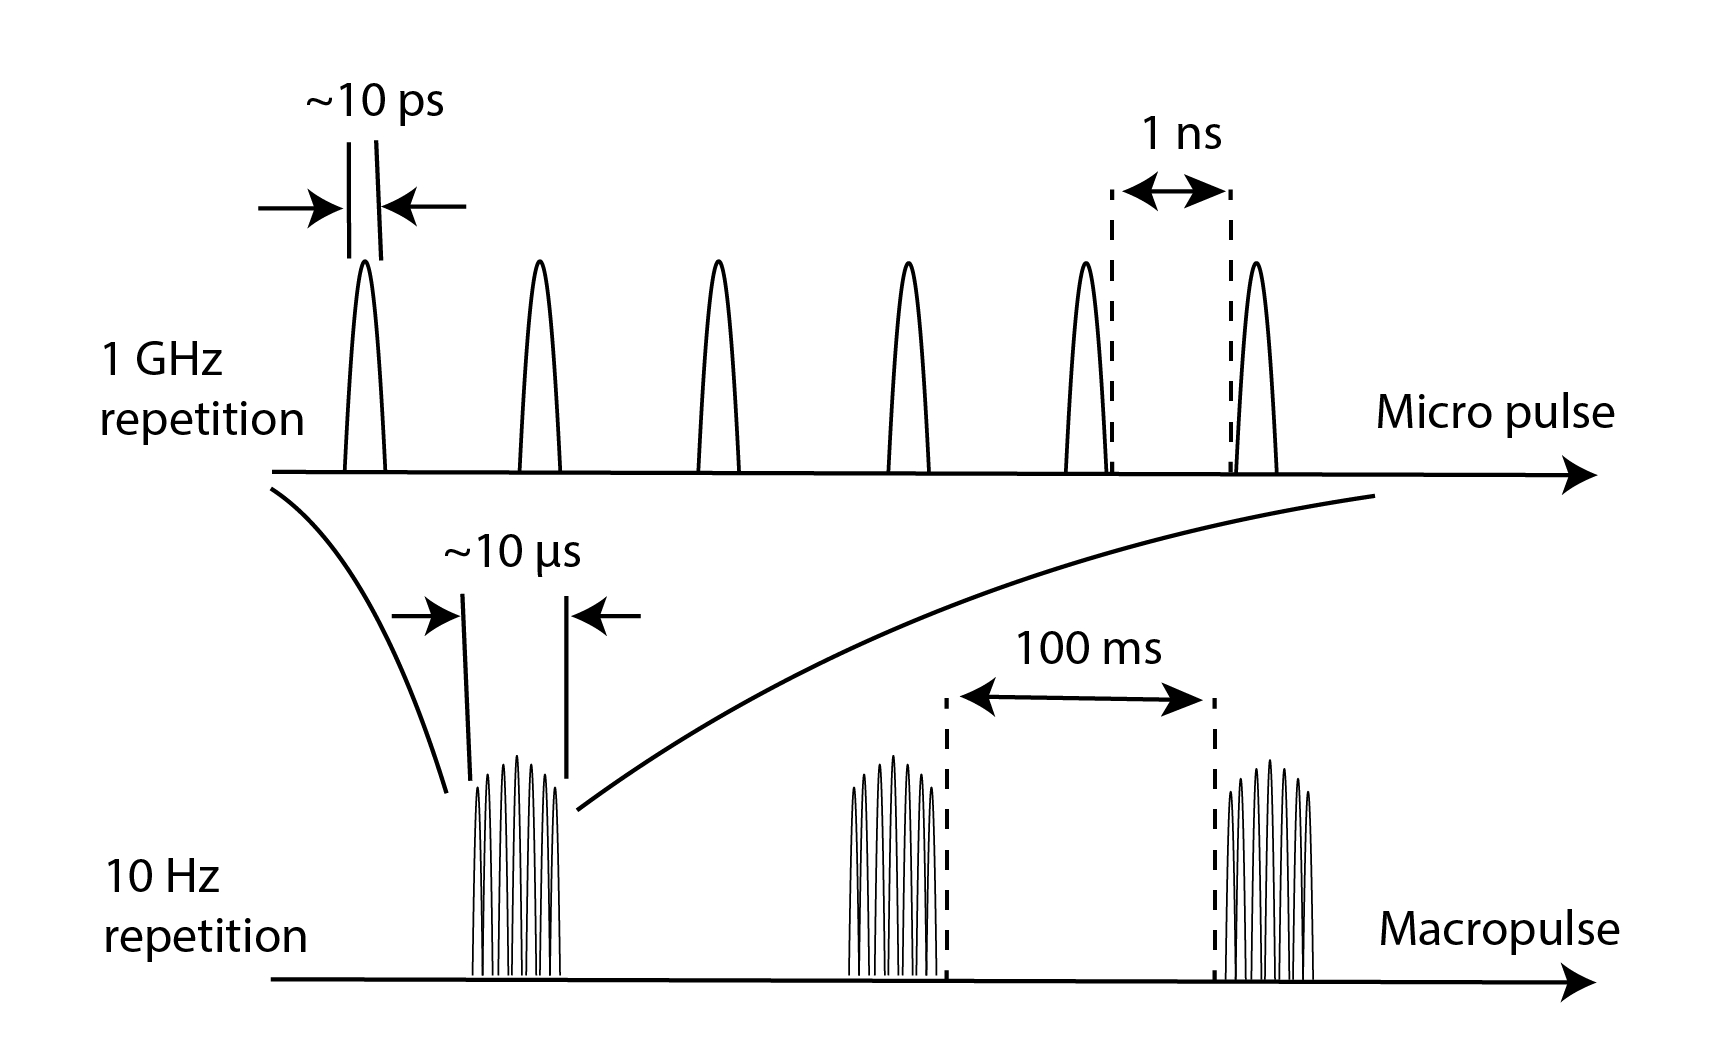
\includegraphics[scale=0.7]{figures/Instruments/FELIX-pulse-02.png}
    \caption{Schematic diagram of the FELIX laser micro and macro pulse structure.}
    \label{fig:FELIX-pulse}
\end{figure}

The maximum macro pulse output power reaching the user station is $> 50$ mJ. The full-width half maxima (FWHM) of radiation is Fourier-transform limited and can be on the order of $\Delta \nu = 5$ \wn\ at 1000 \wn. The schematic drawing of the free-electron laser (FELIX) interfaced with the FELion user station is shown in Figure \ref{fig:FELIX}. At the FELion user station, the IR radiation from FEL-2 is coupled into the FELion via two mirrors (one of them focuses the laser beam into the trap region) and two vacuum windows KRS-5 which permit photons down to 250 \wn\ with 75\% transmission. The KRS-5 windows are replaced with a PPE (beamline exit) and a CVD diamond window (FELion entrance) when FEL-1 is used. The region between the FELIX beamline and FELion is flushed with N$_2$ gas to avoid absorption in air.

\subsubsection{OPO/A}
\label{subsec:ir:radiation-source:OPO}

In addition to the FELIX laser system, the FELion instrument is coupled to a tunable OPO/A system (LaserVision, Narrowband OPO/A model).\\
\\
\textbf{Operating principles:}\\

The OPO/A system uses an optical parametric oscillator (OPO) and amplifier (OPA) 
instead of stimulated emission for optical gain. Hence, it consists of an optical resonator and non-linear crystals. 
It relies on two non-linear optical processes: second harmonic generation (SHG) and difference frequency generation (DFG).

The 1064 nm laser source (pump) input is split using a beam splitter, and one part ($1/3^{rd}$) is directed to the OPO 
stage and the other part ($2/3^{rd}$) to the OPA stage. Before entering the OPO stage, the 1064 nm input is frequency 
doubled via SHG to provide 532 nm input for OPO. In OPO, the input laser beam of frequency $w_p$ is split into two new 
lower energy photons via DFG using KTP crystals, called signal and idler, with frequency $w_s$ and $w_i$, respectively, 
such that $w_p = w_s + w_i$. The wavelengths of $w_s$ and $w_i$ can be tuned by phase-matching conditions (i.e., by 
changing the angle between the incident pump laser and optical axes of crystals). 

While in OPA, in addition to the initial $2/3^{rd}$ of 1064 nm pump beam input ($w_p$), 
the idler output ($w_i$) from OPO acts as a signal input beam for OPA. The signal and pump beam is then directed into
the non-linear KTA crystals of OPA. Subsequently, using DFG, generating high energy output beam 
with a tunable wavelength in the intermediate/mid -infrared region.\\

% Using DFG, the $w_i$ in the mid-infrared region (MIR) is generated. resulting in tunable intermediate/mid-infrared output in the 3 $\mu$m range using DFG.\\
% \\
\textbf{Setup:}\\
The OPO/A system coupled to the FELion instrument is shown as a schematic diagram in Figure \ref{fig:FELIX}. This is a multi-stage nonlinear device designed to convert the fixed-frequency output of a seeded 1064 nm Nd:YAG pump laser (operated at 10Hz) into tunable radiation in the intermediate and mid-infrared, using the combination of a 532 nm pumped OPO followed by a 1064 nm pumped OPA. The system produces a tunable output (MIR Idler) from 2.218-5 $\mu$m, i.e., 2000-4500 \wn\ frequency range with a maximum pulse energy of up to 25 mJ and line bandwidth of $\sim 0.1$ \wn\ (seeded).

